\chapter{Android Application}
\section{Einleitung}

\begin{figure}[H]
\centering
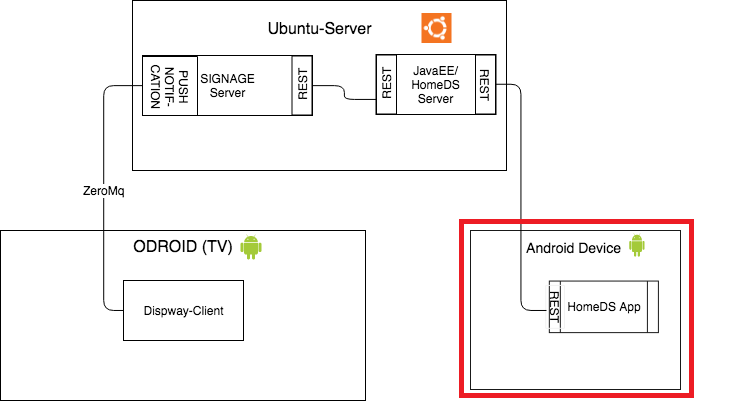
\includegraphics[width=1.0\textwidth]{images/06_AndroidApp/06_SystemArch}
\caption{Die Android Applikation dient zur mobilen Benutzung}
\end{figure}
\\
Um eine höchstmögliche Reichweite an Endgeräten zu erzielen, wurde eine Android Applikation entwickelt, mit der die wichtigsten Funktionen abgedeckt werden. Zum Beispiel das Wechseln der DataSets des XIBO-Servers. Wichtig ist es die Applikation möglichst einfach und leicht bedienbar zu gestalten, um auch Erstbenutzern die Bedienung zu erleichtern. 
Prototyp für die aktuelle Applikation ist eine Anwendung für Android, die direkt mit dem Digital Signage Server kommuniziert. Es stellte sich heraus, dass das Steuern des Servers direkt über eine Applikation auf Android Basis viel zu umständlich ist. Darum wurde eine Browser Applikation entwickelt, welche über das ''HomeDsBackend''(Java-EE-Server) kommuniziert, um das Funktionsspektrum zu erweitern und die Applikation möglichst kompakt zu gestalten. Beispielsweise ist es durch diese Aufteilung nicht mehr nötig eine Datenbank in der Applikation zu haben. Somit erleichtert es auch Applikationen für andere Betriebssysteme zu implementieren. 
\section{Anforderungen}
\\
\begin{figure}[H]
\centering
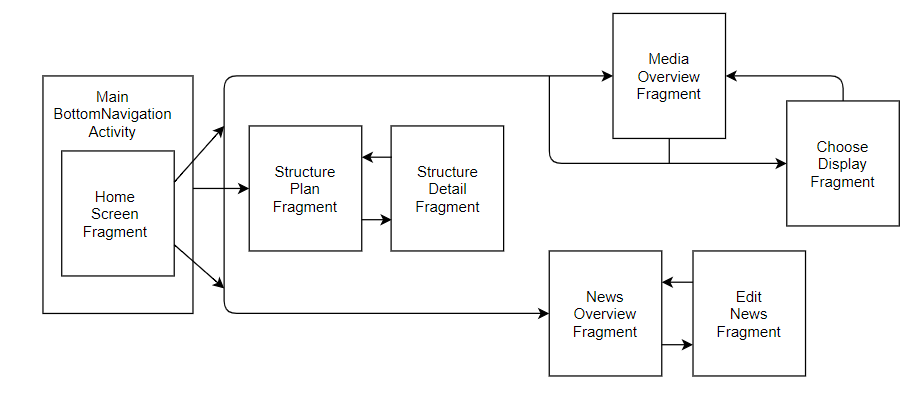
\includegraphics[width=1.0\textwidth]{images/06_AndroidApp/06_AndroidArch}
\caption{Fluss Diagramm der Android Anwendung}
\label{fig:mediaNav}
\end{figure}
\\
Die Anforderungen an die Android Applikation weichen von den Anforderungen an das ''Backend'' leicht ab, da das ''Backend'' die gesamte Zeitsteuerung- und Datenbankfunktionalität übernimmt. Es besteht die Möglichkeit, den Server über die Website des ''Backend'' zu steuern, beziehungsweise über die Applikation auf Android Basis. 
\begin{itemize}
	\item {\em Eilmeldungen:} Dem Benutzer soll es möglich sein Nachrichten in einem Ticker auf den Bildschirmen anzuzeigen.
	
	\item {\em Medien Wiedergabe:} Medien die Lokal am Digital Signage Server liegen sollen abgespielt werden können.
		
	\item {\em Authentifizierung automatisieren (Prototyp Applikation):} Die Authentifizierung am Digital Signage Server soll automatisiert werden, um nicht vom Benutzer durchgeführt werden zu müssen.  		
\end{itemize}
\section{Struktur}
\begin{itemize}
	\item {\em activity:} Alle Activities die für die Anwendung benötigt werden. Als Beispiel die MainActivity
	
	\item {\em adapter:} Hier befinden sich alle Adapter für die RecyclerViews.
	
	\item {\em apiClient:} Beinhaltet die Klasse ''RequestHelper'' mit der die Anfragen an den Digital Signage Server beziehungsweise an das HomeDsBackend vereinfacht werden.
	
	\item {\em entity:} Jene Klassen die als Models für die Anwendung benötigt werden. 
		
	\item {\em enumeration:} Enumerationen welche die Android Basierte Applikation verwendet. Zum Beispiel das ''RequestTypeEnum''.
	
	\item {\em fragment:} Alle Fragments die für das User Interface benötigt werden. Beispiel hierfür ist das Fragment ''NewsOverviewFragment'', welches alle DataSets die am Server sind anzeigt.
	
	\item {\em viewholder:} Beinhaltet alle ''ViewHolder'' die für die verschiedenen ''RecyclerViews'' benötigt werden. 		
\end{itemize}
\section{Benutzerhandbuch}
\subsection{Startseite}
Auf der Einstiegsseite der Applikation ist ein Feld mit dem Serverstatus zu sehen. Sollte dieses Rot eingefärbt sein gibt es Verbindungsprobleme zum Server(die Applikation kann keine Daten vom Server erhalten oder Daten an den Server senden). Andernfalls kann mit der Benutzung fortgefahren werden, der Status wird grün angezeigt. Die Funktion der beiden Buttons wird im weiteren Verlauf des Benutzerhandbuchs erklärt.(Siehe Abbildung \ref{img:onlineOffline})
\\
\begin{figure}[H]
    \centering
    \subfloat{{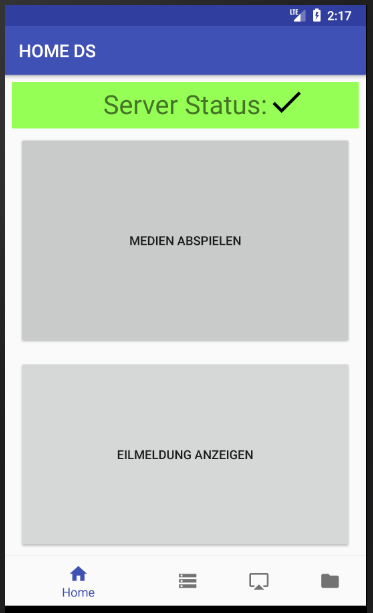
\includegraphics[width=6cm]{images/06_AndroidApp/06_StatusOnline}}}%
    \qquad
    \subfloat{{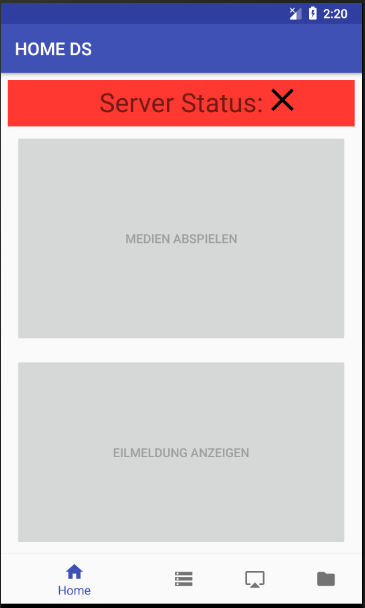
\includegraphics[width=6cm]{images/06_AndroidApp/06_StatusOffline}}}%
    \caption{Startseite mit Status Element Online/Offline}
    \label{img:onlineOffline}
\end{figure}
\\
\subsection{Abspielen von Medien auf gewünschten Bildschirmen}
Das Abspielen von Medien wird im Navigationstab ''Play Media'' abgewickelt. Zusätzlich befindet sich auf der Startseite ein Button über den direkt zu dieser Sektion navigiert werden kann.(Siehe Abbildung \ref{fig:mediaNav})
\\
\begin{figure}[H]
\centering
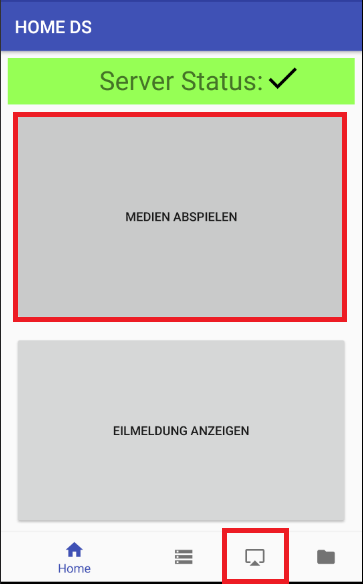
\includegraphics[scale=0.35]{images/06_AndroidApp/06_mediaNavigation}
\caption{Startseite mit markierten Navigationselementen}
\label{fig:mediaNav}
\end{figure}
\\
Wurde noch kein Display gewählt, auf dem das Medium abgespielt werden soll, erscheint zu Beginn eine Auswahlmaske für die Bildschirme die verfügbar sind. Nach Auswahl einer Anzeige navigiert die Applikation automatisch zur Medienübersicht. (Siehe Abbildung \ref{fig:dispNav})
\\
\begin{figure}[H]
\centering
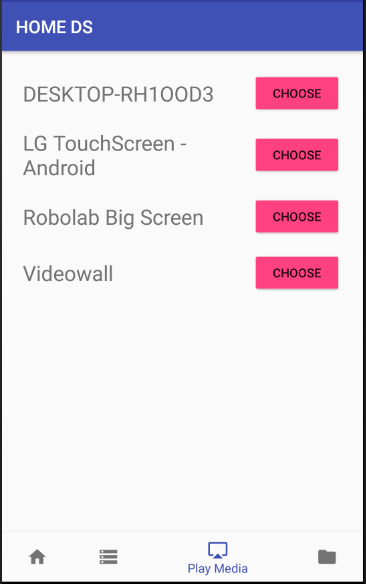
\includegraphics[scale=0.35]{images/06_AndroidApp/06_displayChoice}
\caption{Liste mit verfügbaren Displays}
\label{fig:dispNav}
\end{figure}

Ist bereits ein Bildschirm ausgewählt wird direkt eine Übersicht der abspielbaren Medien angezeigt. Im rechten oberen Teil der Ansicht ist der gewählte Bildschirm zu sehen und über einen Button wird die Bildschirmauswahl angezeigt.(Siehe Abbildung \ref{fig:mediaOv})
\begin{figure}[H]
\centering
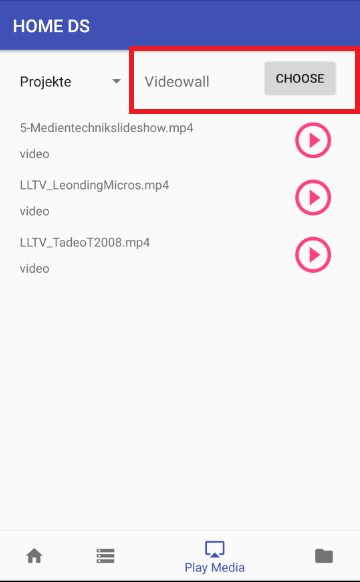
\includegraphics[scale=0.35]{images/06_AndroidApp/06_displayTextAndButton}
\caption{Ausgewählter Bildschirm und Button für die Auswahl}
\label{fig:mediaOv}
\end{figure}
\\
Sortieren der angezeigten Medien ist über einen Spinner im linken oberen Teil der Medienübersicht möglich. Durch Berührung der Anzeigefläche erscheint die Auswahl der Sortiervorschläge.(Siehe Abbildung \ref{fig:spinner})
\begin{figure}[H]
\centering
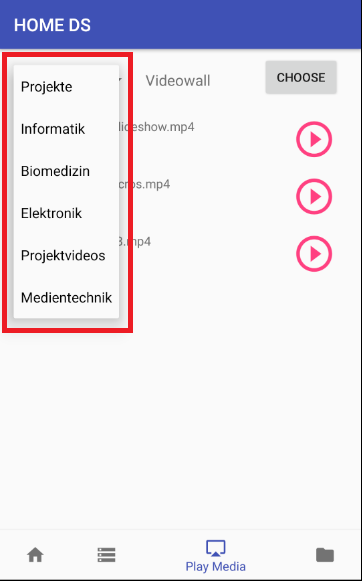
\includegraphics[scale=0.35]{images/06_AndroidApp/06_TagChoice}
\caption{Spinner mit Tags zur Sortierung}
\label{fig:spinner}
\end{figure}
\\
Um ein in der Liste angezeigtes Medium abzuspielen, muss der Play-Button im rechten Teil des Listenelements gedrückt werden. Wird der Button betätigt spielt die gewählte Anzeige das Medium ab .(Siehe Abbildung \ref{fig:playBut})
\begin{figure}[H]
\centering
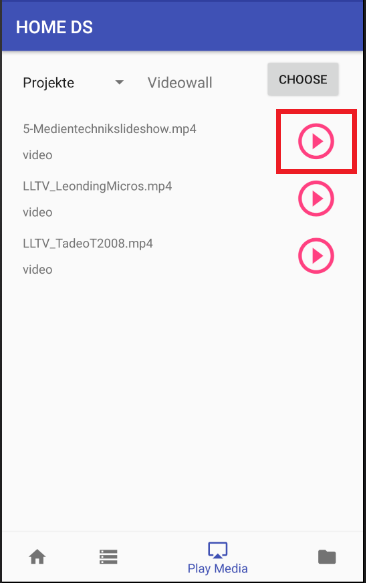
\includegraphics[scale=0.35]{images/06_AndroidApp/06_playMedia}
\caption{Play Button um Medium abzuspielen}
\label{fig:playBut}
\end{figure}
\\
\subsection{Meldungen Anzeigen}
Um eine Meldung anzuzeigen, muss zum ''DataSet'' Tab gewechselt werden. Dies ist auch über eine Schaltfläche auf der Startseite möglich. (Siehe Abbildung \ref{fig:06_dataSetNavigation})
\begin{figure}[H]
\centering
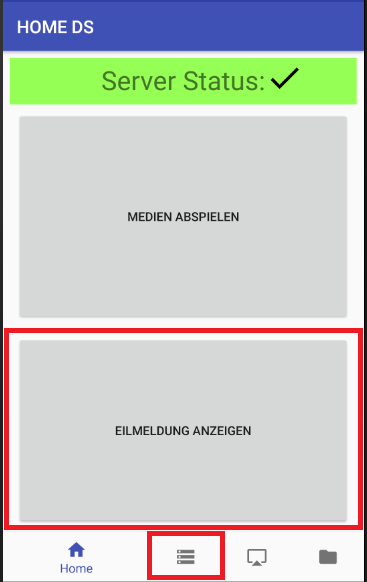
\includegraphics[scale=0.35]{images/06_AndroidApp/06_dataSetNavigation}
\caption{Startseite mit Navigationselementen}
\label{fig:06_dataSetNavigation}
\end{figure}
\\
Die in der Ansicht zu sehende Liste enthält alle aktiven und  inaktiven Meldungen, die auf den Anzeigen wiedergegeben werden beziehungsweise werden können.
(Siehe Abbildung \ref{fig:06_DataSetsToSHow}) 
\\
\begin{figure}[H]
\centering
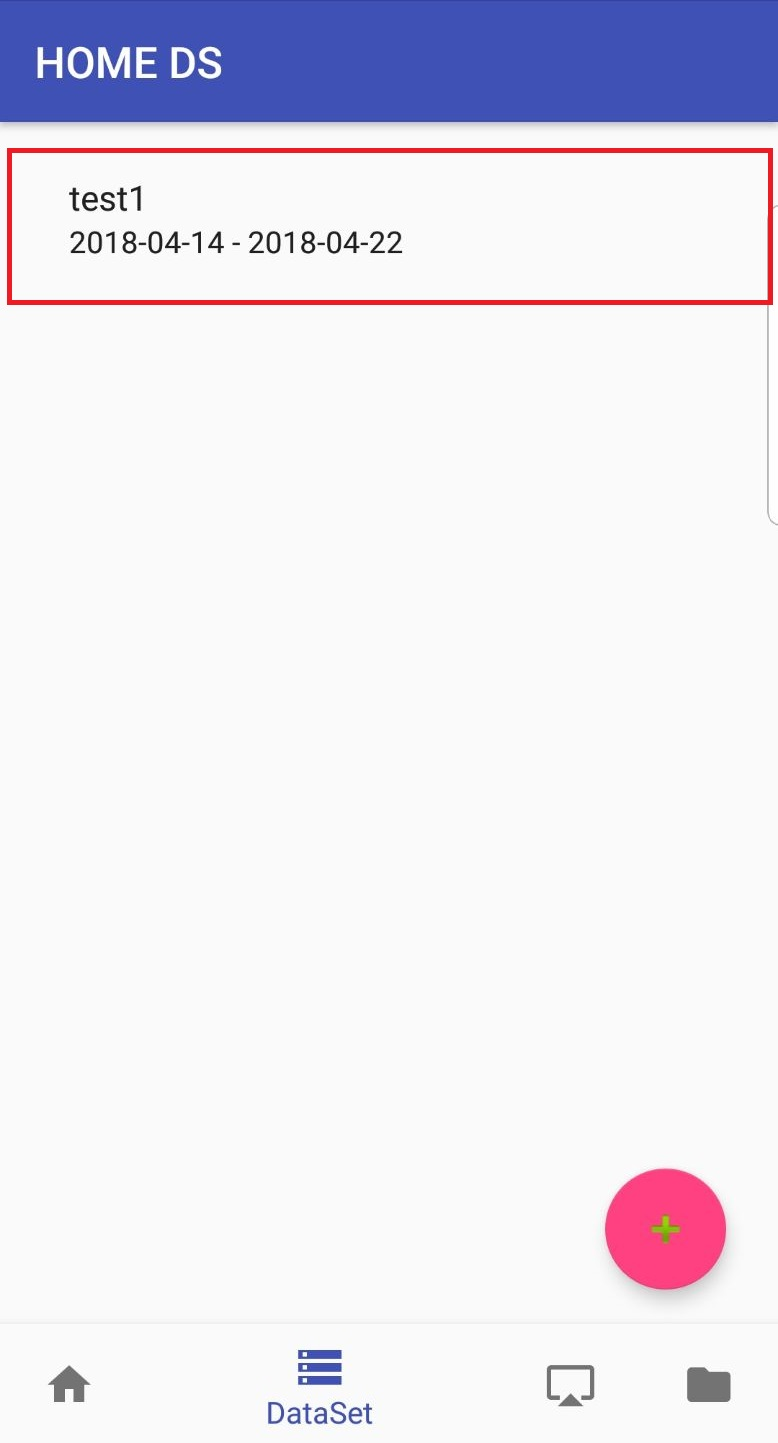
\includegraphics[scale=0.1]{images/06_AndroidApp/06_DataSetsToSHow}
\caption{Am HomeDsBackend vorhandene DataSets}
\label{fig:06_DataSetsToSHow}
\end{figure}

\\
Durch auswählen eines der Listenelemente öffnet sich eine Detailansicht über die die Informationen der Meldung verändert werden können zum Beispiel der Titel oder der Anzeigezeitraum. Wird der FloatingActionButton im unteren rechten Teil der Ansicht gedrückt, so öffnet sich ein Detailfenster welches noch keine Daten eingetragen hat um eine neue Meldung zu erstellen. (Siehe Abbildung \ref{fig:06_NewNewsEdit})
\\
\begin{figure}[H]
    \centering
    \subfloat{{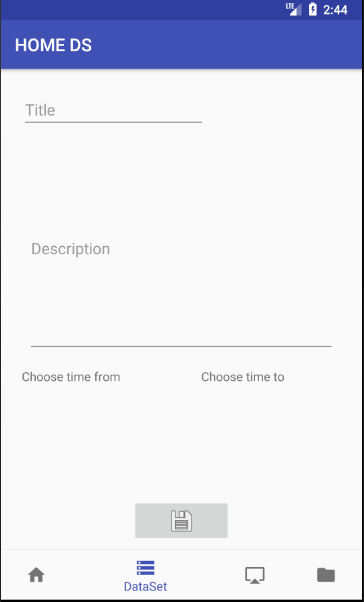
\includegraphics[width=6cm]{images/06_AndroidApp/06_NewNewsEdit}}}%
    \qquad
    \subfloat{{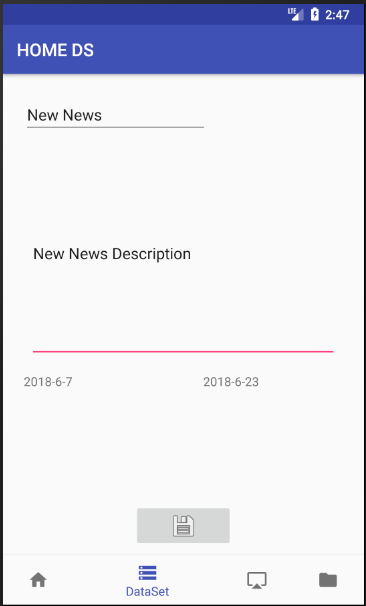
\includegraphics[width=6cm]{images/06_AndroidApp/06_EditNews}}}%
    \caption{Anzeige für ein neues/zu veränderndes DataSet}
    \label{fig:06_NewNewsEdit}
\end{figure}
\\
Vorgenommene Änderungen oder neu erstellte Meldungen können mittels Save Button übernommen werden. Dieser befindet sich im unteren Teil der Detailansicht. Nach dem Speichern einer Meldung navigiert die Applikation wieder auf die Übersicht der Meldungen.(Siehe Abbildung \ref{fig:06_EditNewsSaveButton})

\begin{figure}[H]
\centering
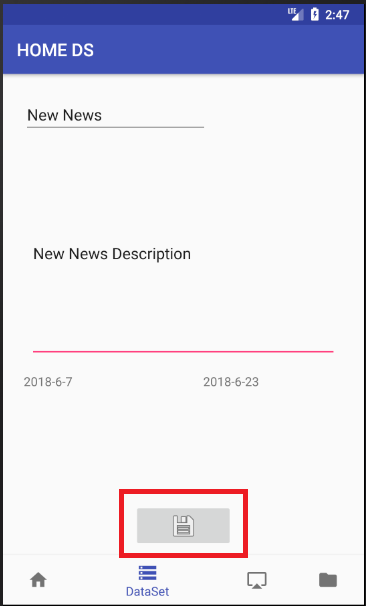
\includegraphics[scale=0.35]{images/06_AndroidApp/06_EditNewsSaveButton}
\caption{Markierter Speichern Button}
\label{fig:06_EditNewsSaveButton}
\end{figure}

\subsection{Strukturübersich}
Ist es nötig eine detaillierte Übersicht über die am Server liegenden Layouts zu bekommen, kann dies über den Navigationstab ''Structure Plan'' getan werden.(Siehe Abbildung \ref{fig:06_EditNewsSaveButton}) 
\\
\begin{figure}[H]
\centering
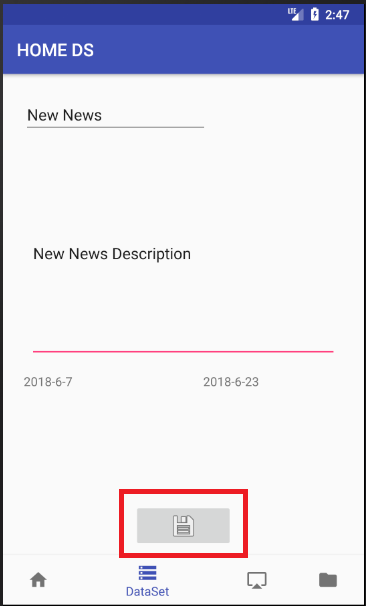
\includegraphics[scale=0.35]{images/06_AndroidApp/06_EditNewsSaveButton}
\caption{Markierte Liste mit Layouts und Navigationstab}
\label{fig:06_EditNewsSaveButton}
\end{figure}
\\
Die Liste zeigt alle am Server befindlichen Layouts. Durch Klicken einer der Listenelemente navigiert die Applikation zu einer Detailansicht des Layouts.(Siehe Abbildung \ref{fig:06_StructureNavigationToDetail})
\\
\begin{figure}[H]
\centering
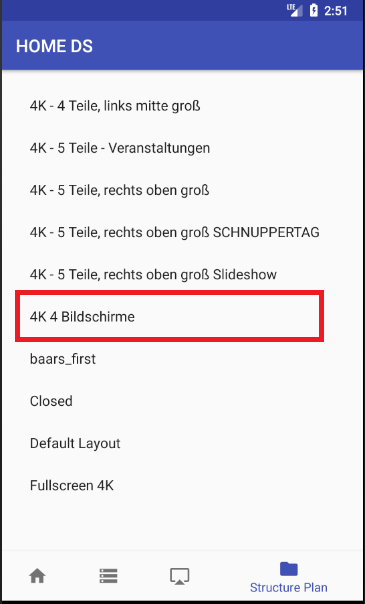
\includegraphics[scale=0.35]{images/06_AndroidApp/06_StructureNavigationToDetail}
\caption{Markiertes Element um auf die Detailansicht zu gelangen}
\label{fig:06_StructureNavigationToDetail}
\end{figure}
\\
Die Detailansicht eines Layouts zeigt die Grunddaten eines Layouts wie zum Beispiel die ID oder die Besitzer ID. Des Weiteren werden alle Unterelemente beispielsweise Widget's angezeigt. Dargestellt wird der JSON-String des Layouts.
(Siehe Abbildung \ref{fig:06_StructureDetail})
\\
\begin{figure}[H]
\centering
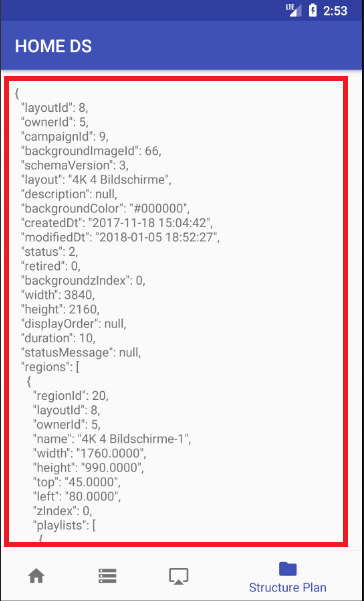
\includegraphics[scale=0.35]{images/06_AndroidApp/06_StructureDetail}
\caption{Markierte Details des Layouts}
\label{fig:06_StructureDetail}
\end{figure}
\\
\section{MainBottomNavigationActivity und OverviewFragment}
\subsection{MainBottomNavigationActivity}
\\
\begin{figure}[H]
\centering
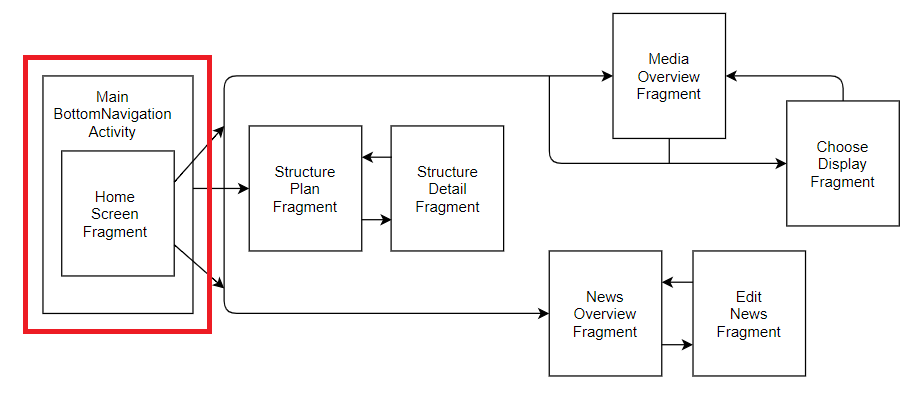
\includegraphics[width=1.0\textwidth]{images/06_AndroidApp/06_AndroidArchMainBottomNavigationActivity}
\caption{Stellung des MainBottomNavigationFragemt in der Android Applikation}
\label{fig:mediaNav}
\end{figure}
\\
Die ''MainBottomNavigationActivity'' ist die einzige ''Activity'' die in der Android Applikation benötigt wird. Hauptaufgabe der ''MainBottomNavigationActivity'' ist es, zwischen den einzelnen ''Fragments'' zu navigieren. Enthalten sind dazu jene Methoden, welche mit dem ''SupportFragmentManager'' die einzelnen Fragments im ''container\_main'' austauschen. Der ''container\_main'' ist ein ''ConstraintLayout'' welches in der zur ''MainActivity'' gehörenden Layout Ressource ''activity\_main.xml'' mit der Identifikationsnummer ''container\_main''  belegt wurde. Zudem wird die Klasse durch das Interface ''AppCompatActivity'' erweitert und implementiert, die ''OnFragmentInteractionListener'' der Fragmente die in der Applikation verwendet werden. 
\
Im unteren Teil der ''Activity'' befindet sich eine Navigationsleiste. Diese ist zuständig für das Wechseln zwischen den einzelnen Fragmenten mit folgenden Navigationspunkten: 

\begin{itemize}
	\item {\em Home:} Jener Menüpunkt der die Startseite der Applikation beinhaltet.
	\item {\em DataSet:} Ist zuständig für die Verwaltung der ''DataSets''.
	\item{\em Medium abspielen:} Beinhaltet die Fragmente die benötigt werden um Medien auf der gewünschten anzeige abzuspielen.
	\item {\em Strukturplan:} Bietet eine Übersicht über die Struktur der am Server liegenden Layouts.
\end{itemize}
\subsubsection{onCreate}
Hier wird die ''MainBottomNavigationActivity'' als ''ContentView'' gesetzt, zudem wird mittels ''SupportFragmentManager'' das ''HomeScreenFragment'' dem ''container\_main'' zugewiesen und angezeigt. Das Feld Display wird neu instantiiert. Die statische Variable ''instance'', vom Datentyp ''MainBottomNavigationActivity'', wird auf die aktuelle Instanz der Klasse zugewiesen. Die ''BottomNavigationBar wird mit Werten belegt und ein ''OnNavigationItemSelectedListener'' gesetzt, um durch die Applikation navigieren zu können.
\begin{lstlisting}[language=Java,caption={Zuweisung von Variablen und Navigationbar}]
setContentView(R.layout.
	activity_main_bottom_navigation);
mainActivityBottomNavigation = this;
openHomeScreenFragment();
display = new Display();
 
navbar = findViewById(R.id.navigation_bar);
navbar.setOnNavigationItemSelectedListener(
	new BottomNavigationView.
   	OnNavigationItemSelectedListener() {
    	@Override
     	public boolean onNavigationItemSelected(
     				@NonNull MenuItem item) {
     		item.setChecked(true);
        	switch (item.getItemId()) {
        		case R.id.editDatasetNavBar:
            		openNewsOverview();
                	break;
            	case R.id.playMediaNavBar:
                	if (display.getDisplay() == null){
                	openChooseDisplayFragment();
                	}else {
                	openMediaOverviewFragment();
                	}
                	break;
            	case R.id.homeScreenNavBar:
                	openHomeScreenFragment();
                	break;
            	case R.id.structurePlanNavBar:
                	openStructurePlanFragment();
                	break;
                	}
          	return false;
        }
	});
\end{lstlisting}	
\subsubsection{getInstance}
 Ist der ''Getter'' für die statische Variable ''instance'' und übergibt die aktuelle Instanz der Klasse.
\begin{lstlisting}[language=Java,caption={Getter für aktuelle Instanz der Activity}]
public static MainActivityBottomNavigation
	 getInstance() {
     return mainActivityBottomNavigation;
}
\end{lstlisting}
\subsubsection{Fragment-Austausch-Methoden}
 Sind jene Methoden, die für das Austauschen der einzelnen ''Fragments'' im ''container\_main'' zuständig sind. Dies geschieht mittels ''SupportFragmentManager'', welcher immer die ''Fragments'' im ''container\_main'' anzeigt und dem ''BackStack'', welcher für die Rückwerts Navigation (mittels retour Knopf des Mobilen Endgerätes) in der Applikation zuständig ist,  hinzufügt. Manche Methoden übergeben zudem noch ein ''Bundle'' an das erstellte ''Fragment'', welches Objekte enthält die im nächsten ''Fragment'' benötigt werden. Erkennungsmerkmal dieser Methoden ist das englische Verb ''open'' am Beginn des Methodennamens. Als Namensbeispiel hierfür wird die Methode ''openNewsEditFragment'' herangezogen.
\begin{lstlisting}[language=Java,caption={Beispiel für Fragment-Austausch-Methode}]
public void openEditNewsFragment(DataSetDataField news) {
Bundle bundle = new Bundle();
bundle.putSerializable("data", news);
NewsEditFragment newsEditFragment =
    new NewsEditFragment();
newsEditFragment.setArguments(bundle);
FragmentManager fm = getSupportFragmentManager();
fm.beginTransaction().replace(
    R.id.container_display, 	
    newsEditFragment,"actEdit")
    .addToBackStack("actEdit").commit();
}
\end{lstlisting}
\subsection{HomeScreenFragment}
\\
\begin{figure}[H]
\centering
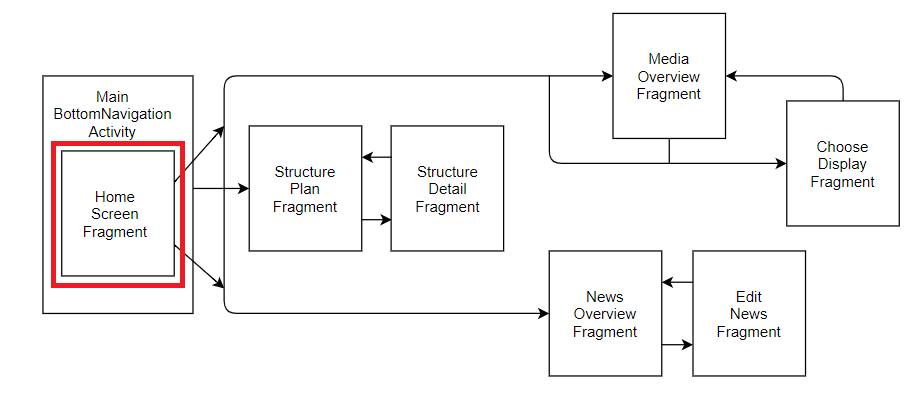
\includegraphics[width=1.0\textwidth]{images/06_AndroidApp/06_AndroidArchHomeScreen}
\caption{Stellung des HomeScreenFragmnet in der Android Applikation}
\label{fig:mediaNav}
\end{figure}
\\
Der Einstiegspunkt der Applikation ist das ''HomeScreenFragment''. Es zeigt den Serverstatus an. Dieser wird über einen ''REST-Request'' vom Java-EE-Server abgefragt. Den Hauptanteil des Fragments bilden die beiden Navigations-Buttons ''Median abspielen'' und ''Eilmeldungen anzeigen''. Durch Klicken dieser Buttons öffnen sich die dazugehörigen Fragmente ''NewsOverviewFragment'' und ''MediaOverviewFragment''.
\\
Die Layout Ressource des ''HomeScreenFragment'' enthält zwei Buttons und ein ''ConstaintLayout''. Dieses ''ConstraintLayout'' beinhaltet wiederum eine ''TextView'' und zwei ''ImageViews''. In der ''onCreate'' Methode des Fragments werden als erstes die Anzeigeelemente neu deklarierten Variablen zugewiesen und im ''ConstraintLayout'' wird der Serverstatus auf View standardmäßig als Offline angezeigt und die Buttons deaktiviert.
\begin{lstlisting}[language=Java,caption={Initialisieren der Variablen im HomeScreenFragment }]
Button btPlayMedia = v.findViewById(R.id.btPlayMedia);
Button btShowNews = v.findViewById(R.id.btShowNews);

btPlayMedia.setEnabled(false);
btShowNews.setEnabled(false);
    
ImageView ivUp = v.findViewById(R.id.ivServerUp);
ivUp.setVisibility(View.INVISIBLE);
    
ImageView ivDown = v.findViewById(R.id.ivServerDown);    
ivDown.setVisibility(View.VISIBLE);
    
ConstraintLayout clServerStatus = 
    v.findViewById(R.id.cl_serverStatus);
clServerStatus.setBackgroundColor(
    ContextCompat.getColor(
    this.getContext(), R.color.serverDown));
}
\end{lstlisting}
Im folgenden Schritt wird über einen ''GET-Request'' die Uhrzeit des XIBO-Servers über den Java-EE-Server abgefragt. Wird die Uhrzeit erhalten, so wird im ''ConstraintLayout'' der Server Status auf online gesetzt und das dazugehörige Bild angezeigt und die Buttons werden freigegeben. Erhält man keine Antwort bleibt die Anzeige unverändert.

\begin{lstlisting}[language=Java,caption={Status Request im HomeScreenFragment}]
rh.executeRequest(RequestTypeEnum.GET, null,
	MainActivityBottomNavigation.getInstance()
	.url + "/status/", () -> {   
    MainActivityBottomNavigation.getInstance()
    .runOnUiThread(() -> {
      	if (rh.getResponseCode() == 200) {
        	
           	ivUp.setVisibility(View.VISIBLE);
            ivDown.setVisibility(View.INVISIBLE);
                
            clServerStatus.setBackgroundColor(
           	ContextCompat.getColor(this.getContext(),
           	R.color.serverUp));
                	
            btPlayMedia.setEnabled(true);
            btShowNews.setEnabled(true);
                    
         }else {
         	ivDown.setVisibility(View.VISIBLE);
                    
            clServerStatus.setBackgroundColor(
            	ContextCompat.getColor(this.getContext(),
                R.color.serverDown));
            }
    });
});
\end{lstlisting}
Um die Navigation über die erstellten Buttons zu ermöglichen wird, ein ''OnClickListener'' Implementiert.
\begin{lstlisting}[language=Java,caption={OnClickListener für die direkte Navigation über Buttons im HomeScreenFragment}]
btPlayMedia.setOnClickListener(
	new View.OnClickListener() {
            
    	@Override
        public void onClick(View view) {
            MainActivityBottomNavigation.
            getInstance().navbar
            .setSelectedItemId(R.id.playMediaNavBar);
        }
     });
\end{lstlisting}
\section{DataSet Verwaltung}
\\
\begin{figure}[H]
\centering
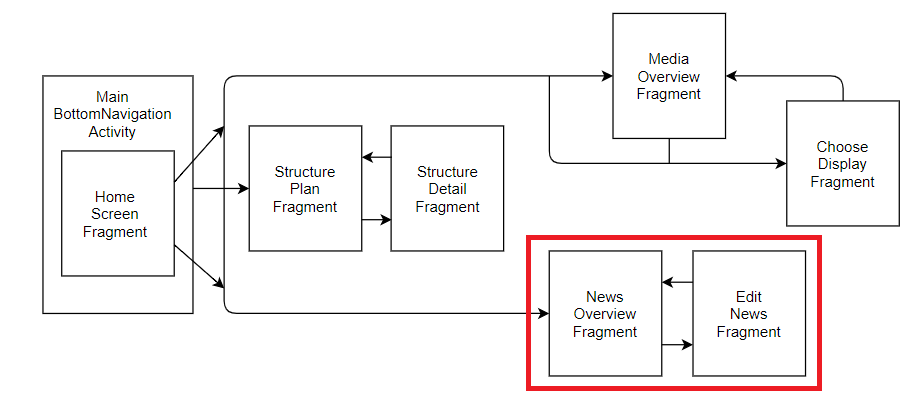
\includegraphics[width=1.0\textwidth]{images/06_AndroidApp/06_AndroidArchShowNews}
\caption{Stellung der DataSet Verwaltung in der Android Applikation}
\label{fig:mediaNav}
\end{figure}
\\
Die beiden Fragmente  ''NewsOverviewFragment'' und ''NewsEditFragment'' sind für die Verwaltung der ''DataSets'' zuständig. Im Fragment ''NewsOverviewFragment'' wird eine Übersicht über alle vorhandenen ''DataSets'' gegeben. Das ''NewsEditFragment'' Fragment wird verwendet, um vorhandene ''DataSets'' zu bearbeiten oder neue ''DataSets'' zu erstellen. 
\subsubsection{NewsOverviewFragment}
Dieses Fragment zeigt alle aktiven ''DataSets'' an. Diese werden vom Server bereitgestellt und per ''REST-Request'' abgefragt. Über einen ''FloatingActionButton'' kann ein neues ''DataSet'' erstellt werden. Durch Klicken auf eines der Listen Elemente, öffnet sich eine Detailansicht in der das Bearbeiten, eines des ''DataSets'' möglich ist.
\\
\begin{figure}[H]
\centering
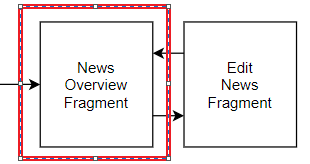
\includegraphics[width=1.0\textwidth]{images/06_AndroidApp/06_NewsOverviewStellung}
\caption{Stellung des NewsOverViewFragment in der Android Applikation}
\label{fig:mediaNav}
\end{figure}
\\
Die Layout Ressource des Fragments, ''fragment\_news\_overview.xml'' enthält eine ''RecyclerView'' und einen ''FloatingActionButton''. Die Logik der Anzeige ist in der Java Klasse ''NewsOverviewFragment'' implementiert. Die meisten Methoden dieser Klasse werden generisch beim Erstellen eines Fragments erzeugt. Die einzige Methode die überschrieben wurde, ist die Methode ''onCreateView''. Beim Ausführen dieser Methode wird zuerst eine ''View'' erstellt welche das ''fragment\_news\_overview'' Layout zugewiesen bekommt. Anschließend wird eine ''RecyclerView'' und ein ''FlaootingActionButton'' erstellt und den zugehörigen Anzeige Elementen zugewiesen.
\begin{lstlisting}[language=Java,caption={Zuweisungen von Variablen und FloatingActionButton-OnClickListener des NewsOverviewFragment }]
View v = inflater.inflate(
	R.layout.fragment_news_overview, container, false);
RecyclerView rv = v.findViewById(R.id.rvNews);

FloatingActionButton fabAddNews = 
    v.findViewById(R.id.fabAddNews);

\end{listings}
 Der ''FlaootingActionButton'' erhält einen ''OnClickListener'' über diesen wird in der ''MainActivity'' eine Methode aufgerufen die ein neues ''NewsEditFragment'' anzeigt, um ein neues ''DataSet'' zu erstellen. 
 \begin{listings}[language=Java, caption={}
fabAddNews.setOnClickListener(
	new View.OnClickListener() {
        @Override
        public void onClick(View view) {
            MainActivityBottomNavigation.
            getInstance().
            openEditNewsFragment(
            new DataSetDataField());
        }
    });
\end{lstlisting}
Um in der ''RecyclerView'' Elemente anzeigen zu können werden diese über einen REST-Request an den Server abgefragt und der ''RecyclerView'' übergeben.
\begin{lstlisting}[language=Java,caption={Anzeigen der abgefragten Elemente im NewsOverviewFragment}]
rh.executeRequest(RequestTypeEnum.GET, null,
	MainActivityBottomNavigation
	.getInstance().url 
	+ "/datasetdatafield/", () -> {

        MainActivityBottomNavigation.getInstance()
        .runOnUiThread(() -> {
            //Belegung der angezeigten Elemente
        });
    });
\end{lstlisting}
\subsubsection{NewsEditFragment}
\\
\begin{figure}[H]
\centering
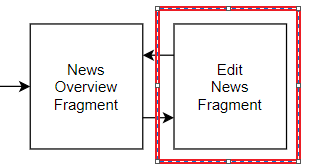
\includegraphics[width=1.0\textwidth]{images/06_AndroidApp/06_NewsEditStellung}
\caption{Stellung des NewsEditFragment in der Android Applikation}
\label{fig:mediaNav}
\end{figure}
\\
Das Fragment zeigt alle Details eines ''DataSets'' an und bietet die Möglichkeit die Detailinformationen bearbeiten zu können. Ebenso wird dieses Fragment dazu verwendet, ein neues ''DataSet'' zu erstellen. Dazu wird das Fragment mit Hinweisen auf die Eingabeoptionen erstellt. Über einen Button können die eingegeben Felder an den ''Java-EE-Server'' übermittelt werden. Eingabe Felder:
\begin{itemize}
	\item {\em Titel:} Das Feld ''Titel'' beinhaltet die Überschrift der anzuzeigenden Information.
	\item {\em Beschreibung:} Hier wird der eigentliche Informationstext eingefügt.
	\item{\em Datum-Von-Bis:} Diese Felder werden über ein ''DatePickerDialog'' befüllt, welcher einen Kalender öffnet und zeigen an in welchem Zeitraum das ''DataSet'' angezeigt wird. 
	\item {\em Uhrzeit-Von-Bis:} Die Anzeige Elemente geben Auskunft über die Zeitspanne in der das ''DataSet'' an den einzelnen Tagen angezeigt wird. Das Feld kann mittels ''TimePickerDialog'' befüllt werden.		
\end{itemize}
Anzeige Ressourcen für dieses Fragment werden in der Datei ''fragment\_news\_edit.xml'' bereitgestellt. Diese enthält die benötigten Tags, um die im oberen Teil beschrieben Eingabefelder zur Verfügung zu stellen. Die Verwendung und Belegung dieser Felder wird in der Klasse ''NewsEditFragment'' implementiert. Auch in dieser Klasse wird  nur die Methode ''onCreateView'' mit Quellcode versehen. Zu Beginn wird der deklarierten ''View'' die ''fragment\_news\_edit.xml'' als Ressource zugewiesen. Um Daten aus dem ''NewsOverviewFragment'' zu empfangen, wird ein ''Bundle'' befüllt. Wenn das befüllte ''Bundle'' Informationen beinhaltet, dann wird die Funktion ''setArguments'' der Basisklasse Fragment(android.support.v4.app.Fragment) mit dem Parameter ''bundle'' aufgerufen, um das Feld ''mArguments'' der Basisklasse Fragment mit Daten zu versehen(Vererbung). Die zuvor deklarierten Variablen (benötigte ''Views'') werden jetzt initialisiert.
\begin{lstlisting}[language=Java,caption={Übernahme der übergebenen Werte und initialisieren der Variablen im NewsEditFragment }]
Bundle bundle = getArguments();
Log.d("BUNDLDATA", String.valueOf(bundle));
if (bundle != null){
    this.setArguments(bundle);
    }
            
DataSetDataField news =
 	(DataSetDataField) bundle.getSerializable("data");
ImageButton ibSaveNews =
  	v.findViewById(R.id.ibSaveNews);
        
title = v.findViewById(R.id.etTitle);
description = v.findViewById(R.id.etDescription);

title.setText(news.getTitle());
description.setText(news.getValue());

tvTimeFrom = v.findViewById(R.id.tvTimeFrom);
tvTimeTo = v.findViewById(R.id.tvTimeTo);
\end{lstlisting}

Das Fragment hat zwei verschiedene Vorgehensweisen. Zum einen werden, sollte ein ''DataSet'' in Form eines ''Bundels'' übergeben werden, die Anzeigeelemente mit den übergebenen Werten befüllt. Andernfalls werden die Felder mit keinen Werten versehen, es werden Hinweise auf die Eingabeoptionen im aktuellen Fragment angezeigt.

\begin{lstlisting}[language=Java,caption={Bedingung für Fragment-Recycling im NewsEditFragment}]
if (news.getToDate() != null 
		&& news.getFromDate() != null) {
    tvTimeFrom.setText(news.getFromDate().toString());
    tvTimeTo.setText(news.getToDate().toString());
    dateTo = news.getToDate();
    dateFrom = news.getFromDate();
}   
\end{lstlisting}

Die benötigten ''onClickListener'' für die Datum- und Uhrzeiteingaben werden im Anschluss implementiert und mittels ''DatePickerDialog'' beziehungsweise ''TimePickerDialog'' mit Daten versehen. 
\begin{lstlisting}[language=Java,caption={OnClickListener für Datum-Auswahl im NewsEditFragment}]
tvTimeTo.setOnClickListener(new View.OnClickListener() {
	@Override
    public void onClick(View view) {
    	final Calendar c = Calendar.getInstance();
        year = c.get(Calendar.YEAR);
        month = c.get(Calendar.MONTH);
        day = c.get(Calendar.DAY_OF_MONTH);

        DatePickerDialog datePickerDialog = 
        	new DatePickerDialog(
            MainActivityBottomNavigation.getInstance()
            , new DatePickerDialog.OnDateSetListener() {
            	@Override
                public void onDateSet(
                  		DatePicker datePicker,
                   		int year, int month, int day) {
                	tvTimeTo.setText(year + "-" 
                        			+ (month + 1)
                        			+ "-" + day);
                    dateTo = LocalDate.
                    	of(year, month, day);
                }
            }, year, month, day);
            datePickerDialog.show();
        }
    });
\end{lstlisting}

Durch Drücken des Buttons(Speicher Button) wird ein Event ausgelöst. Dieses Event kann zwei verschiedene Ausgänge haben: Wenn das im Event erhaltene ''Bundle'' eine ''ID'' besitzt, lässt sich daraus eindeutig schließen, ob es sich hierbei um ein Dataset handelt, das vom User erstellt wurde, oder um eines, das bereits zuvor am Java-EE-Server vorhanden war, indem man überpfrüft, ob die im Bundle enthaltene Information ''ID'' den Wert null hat, oder nicht. Falls dies nämlich der Fall ist, sind es eindeutig vom Benutzer eingegebene Daten. Somit muss deswegen am Server anschließend ein ''POST-Request'' durchgeführt werden, um die neu erstellten Informationen zu senden.
Wenn es ein vom Java-EE-Server erhaltenes ''DataSet'' ist, wird stattdessen ein ''PUT-Request'' durchgeführt, der die veränderten Daten übermittelt. 
\begin{lstlisting}[language=Java,caption={Unterscheidung der Art der Anfrage im NewsEditFragment}]
if (news.getId() != null && news.getDataSetId() 
		!= null && news.getDataRowId() != null) {
	params.put("id", news.getId().toString());
    params.put("dataSetId", news.getDataSetId().toString());
    params.put("dataRowId", news.getDataRowId().toString());
   } 
       
if (news.getId() == null) {
    Long n = -1L;
    params.put("dataRowId", n.toString());
    rh.executeRequest(RequestTypeEnum.POST, params,
       	MainActivityBottomNavigation
        .getInstance().url + "/datasetdatafield/save/",
         () -> {
          //Toast ausgabe
        });
}  else {
    rh.executeRequest(RequestTypeEnum.PUT, params,
        MainActivityBottomNavigation
        .getInstance().url + "/datasetdatafield/edit/",
       	() -> { 
          //Toast ausgabe
        });                 
    }
\end{lstlisting} 
\section{Mediaplayer}
\\
\begin{figure}[H]
\centering
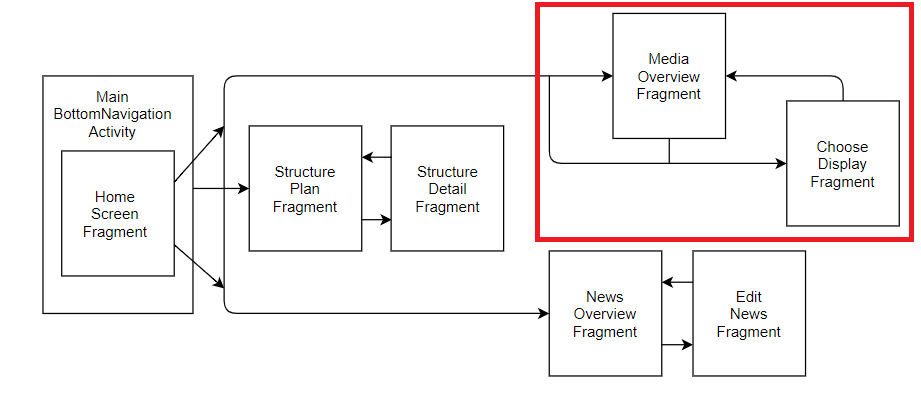
\includegraphics[width=1.0\textwidth]{images/06_AndroidApp/06_AndroidArchPlayMedia}
\caption{Stellung der Media Navigation in der Android Applikation}
\label{fig:mediaNav}
\end{figure}
\\
Um auf einer gewünschten Anzeige ein, sich auf dem Server befindliches, Medium abzuspielen, werden die beiden Fragments ''MediaOverViewFragment'' und ''ChooseDisplayFragment'' implementiert. Das gewünschte Medium wird auf dem ausgewählten Display sofort abgespielt. Ist noch kein Display ausgewählt, wird man zuerst auf das ''ChooseDisplayFragment'' geleitet, um einen Bildschirm zu wählen.
\subsubsection{MediaOverviewFragment}
Im diesem Fragment werden alle Medien angezeigt, die sich am XIBO-Server in der Bibliothek befinden und mit dem richtigen Tag markiert sind. Eine Sortierung der Liste ist über ein ''Spinner'' Element möglich. Des Weiteren wird im rechten oberen Teil des Fragments der Display angezeigt, auf dem das gewählte Medium abgespielt werden soll. Eine Auswahl des Displays ist über Navigation zum ''ChooseDisplayFragment'' möglich, dieses wird über den Button ''Auswählen'' geöffnet. Hat der Benutzer noch keinen Display ausgewählt wird er zuerst auf das ''ChooseDisplayFragment'' weitergeleitet.
\\
\begin{figure}[H]
\centering
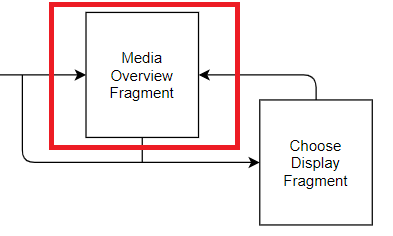
\includegraphics[width=1.0\textwidth]{images/06_AndroidApp/06_MediaOverViewStellung}
\caption{Stellung des MediaOverViewFragment in der Android Applikation}
\label{fig:mediaNav}
\end{figure}
\\
Durch die Ressource Datei ''fragment\_media\_overview.xml'' können die Elemente in der View angezeigt werden. Dieses Layout beinhaltet neben einer ''RecyclerView'' zur Darstellung der abzuspielenden Medien zwei Buttons, eine TextView und einen Spinner zur Sortierung der angezeigten Liste. Einstiegspunkt der Methode ''onCreateView'' ist die Zuweisung der Layout Ressource. Zusätzlich werden die in der Klasse deklarierten Variablen mit den Anzeigeelementen verknüpft. Die TextView wird im Anschluss mit dem Namen des, für die Wiedergabe gewählten Displays, belegt.
\begin{lstlisting}[language=Java,caption={Instantiieren der benötigten Variablen im MediaOverviewFragment}]
View v = inflater.inflate(
	R.layout.fragment_media_overview, container, false);
rvMedia = v.findViewById(R.id.rvMedia);
medias = new LinkedList<>();
spTagChoise = v.findViewById(R.id.spTagChoise);
btCooseDisplay = v.findViewById(R.id.btChooseDisplay);
tvDisplayToPlay = v.findViewById(R.id.tvDisplayToPlay);
tvDisplayToPlay.setText(
	MainActivityBottomNavigation.getInstance()
	.getDisplay().getDisplay()); 
\end{lstlisting}
Um die Liste der Medien zu sortieren, wird ein ArrayAdapter initialisiert. Diesem werden die Ressourcen ''tag\_array'', beinhaltet eine Liste mit Sortiermöglichkeiten für die angezeigten Medien, und ''simple\_spinner\_item'' um das Design für die angezeigten ''Spinner'' Elemente, übergeben. Es erfolgt eine Zuweisung des Adapters an das Spinner Element. Um die Sortierung der Medien Liste zu realisieren, wird ein ''OnItemSelectedListener'' implementiert der die Medien gefiltert nach ausgewähltem Tag anzeigt. Um zu Beginn alle Inhalte anzuzeigen, wird dem Spinner das erste Element des ''tag\_array'' als Standardsortierung zugewiesen.
\begin{lstlisting}[language=Java,caption={Erstellen des Spinner und der dazugehörigen Event-Listener MediaOverviewFragment}]
ArrayAdapter<CharSequence> tagAdapter =
	ArrayAdapter.createFromResource(
    MainActivityBottomNavigation.getInstance()
    .getApplicationContext(), R.array.tag_array,
    android.R.layout.simple_spinner_item);
        
tagAdapter.setDropDownViewResource(
	android.R.layout.simple_spinner_dropdown_item);
    	
spTagChoise.setAdapter(tagAdapter);
spTagChoise.setOnItemSelectedListener(
	new AdapterView.OnItemSelectedListener() {
        @Override
        public void onItemSelected(AdapterView<?> adapterView,
        						 View view, int i, long l) {
            mediaTag = adapterView
            	.getItemAtPosition(i).toString();
            setRecyclerView(mediaTag,rvMedia);
        }
        @Override
        public void onNothingSelected(AdapterView<?> adapterView) {
            spTagChoise.setSelection(0);
            mediaTag = adapterView.getItemAtPosition(0).toString();
            setRecyclerView(mediaTag,rvMedia);
        }
    });
spTagChoise.setSelection(0);

mediaTag = spTagChoise.getItemAtPosition(0).toString();
\end{lstlisting}
Um zwischen den einzelnen Displays zu wählen, wird dem ''Auswählen'' Button ein ''onClickListener'' zugewiesen welcher die Navigation zum ''ChooseDisplayFragment'' einleitet.

\begin{lstlisting}[language=Java,caption={OnClickListener für Displayauswahl im MediaOverviewFragment}]
btCooseDisplay.setOnClickListener(new View.OnClickListener() {
   	@Override
    public void onClick(View view) {
    	MainActivityBottomNavigation
    	.getInstance().openChooseDisplayFragment();
      	
        tvDisplayToPlay.setText(
        	MainActivityBottomNavigation.getInstance()
        	.getDisplay().getDisplay());
        }
    });
\end{lstlisting}

Des Weiteren wird die Methode ''setRecyclerView'' erstellt, um die Daten nach Tag sortiert, vom Server mittels ''GET-Request'' zu erhalten und diese auf der View anzeigen zu können.


\begin{lstlisting}[language=Java,caption={Anfordern und anzeigen der Daten vom Server im MediaOverviewFragment}]
HashMap<String, String> params = new HashMap<>();
params.put("start", "1");
params.put("length", "10");
params.put("tags", mediaTag);
        
rh.executeRequest(RequestTypeEnum.GET, params, 										MainActivityBottomNavigation.getInstance()
    .url + "/media/", () -> {
    	MainActivityBottomNavigation.getInstance()
    	.runOnUiThread(() -> {
			//Belegung der angezeigten Elemente            
		});
\end{lstlisting}
\subsubsection{ChooseDisplayFragment}
Die Auswahl des Bildschirmes auf dem das Medium angezeigt werden soll erfolgt über dieses Fragment. Dazu werden die verfügbaren Displays vom Java-EE-Server abgefragt und in einer Liste angezeigt. Durch Klicken auf den ''Auswählen'' Button in einem der in der Liste angezeigten Display Elementen, wird dieser Display ausgewählt und Medien werden dann auf diesem abgespielt. 
\\
\begin{figure}[H]
\centering
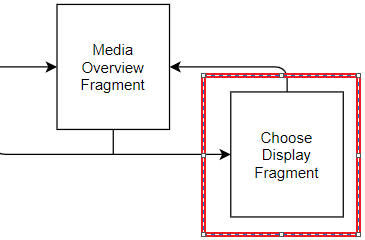
\includegraphics[width=1.0\textwidth]{images/06_AndroidApp/06_ChooseDisplayStellung}
\caption{Stellung des ChooseDisplayFragment in der Android Applikation}
\label{fig:mediaNav}
\end{figure}
\\
Die RecyclerView Ressource, um die zu wählenden Displays anzuzeigen ist in der Datei ''fragment\_choose\_display.xml'' angelegt. Zuweisen der Layout Ressource auf die aktuelle View, initialisieren der Klassen Attribute und aufrufen der Methode ''getDisplays'' sind die einzigen Schritte der ''onCreateView'' Funktion.''getDisplays'' ist jene Methode die alle Displays, die mit dem XIBO-Server verbunden sind, per ''GET-Request'' abfragt beziehungsweise aufbereitet und der RecyclerView übergibt, um diese auf der View anzuzeigen. 
\begin{lstlisting}[language=Java,caption={Abfragen und anzeigen der Displays im ChooseDisplayFragment}]
rh.executeRequest(RequestTypeEnum.GET, null,					MainActivityBottomNavigation.getInstance().
	url + "/display/", () -> {
		//Belegung der angezeigten Elemente
	});
\end{lstlisting}
\section{Strukturplan}
\\
\begin{figure}[H]
\centering
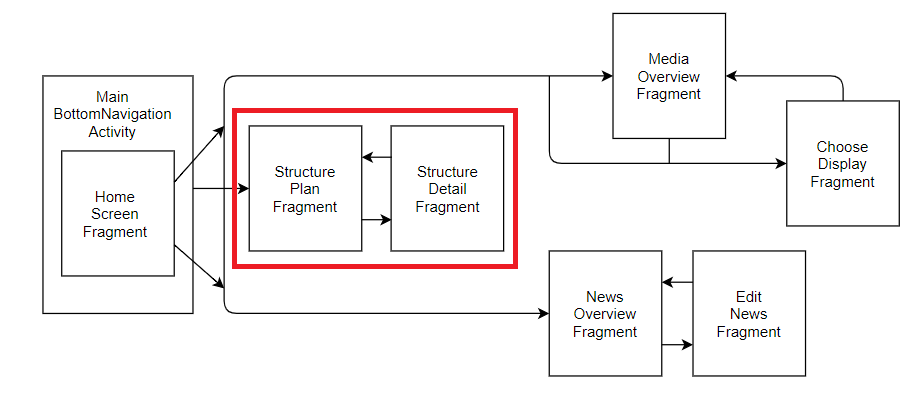
\includegraphics[width=1.0\textwidth]{images/06_AndroidApp/06_AndroidArchStructureCrawler}
\caption{Stellung der Strukturverwaltung in der Android Applikation}
\label{fig:mediaNav}
\end{figure}
\\	
Die am XIBO-Server liegenden Layouts werden in der Andoid Applikation formatiert als ''JSON-Sting'' angezeigt. Damit ist gewährleistet, dass der App-Benutzer eine Übersicht über die Struktur der einzelnen Layouts und deren Unterelementen zur Verfügung hat.
\subsubsection{StructurePlanFragment}
Dieses Fragment zeigt eine Übersicht der einzelnen Layouts in Form einer Liste an. Durch Klicken der einzelnen Listen Elemente navigiert die Applikation zu einer Detailansicht über das gewählte Layout.
\\
\begin{figure}[H]
\centering
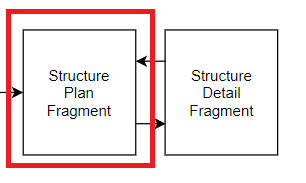
\includegraphics[width=1.0\textwidth]{images/06_AndroidApp/06_StructurePlanStellung}
\caption{Stellung des StructurePlanFragment in der Android Applikation}
\label{fig:mediaNav}
\end{figure}
\\	
Die Ressource zur Gestaltung der Anzeige beinhaltet eine ''RecyclerView'' und heißt ''fragment\_structure\_plan.xml''. Zu Beginn der ''onCreateView'' Methode wird zuerst eine ''View'' erstellt welche das ''fragment\_structure\_plan.xml'' Layout zugewiesen bekommt. Die ''RecyclerView'' wird anschließend initialisiert und über einen ''GET-Request'', dessen Response die einzelnen Layouts und deren Unterstrukturen,des Xibo-Servers in Form eines JSON-Strings übermittelt, befüllt. Somit ist auf der Anzeige eine Liste mit auswählbaren Layouts vorhanden über die zu einer Detailansicht navigiert werden kann. 
\begin{lstlisting}[language=Java,caption={Abfrage und anzeigen der Daten im StructurePlanFragment}]
RecyclerView rvStructurePlan = v.findViewById(R.id.rvStructurePlan);
HashMap<String,String> params = new HashMap<>();
params.put("layoutId","-1");
    
rh.executeRequest(RequestTypeEnum.GET,params
	,MainActivityBottomNavigation.getInstance()
	.url + "/crawler/", ()->{
		//Belegung der angezeigten Elemente
		}
\end{lstlisting}

\subsubsection{StructureDetailFragment}
Ein Layout wird in diesem Fragment in Form eines ''JSON-Strings'' mit allen dazugehörigen Unterelementen angezeigt. Wichtig hierbei ist es den angezeigten ''JSON-String'' richtig zu formatieren, um die Übersichtlichkeit bei zu behalten.
\\
\begin{figure}[H]
\centering
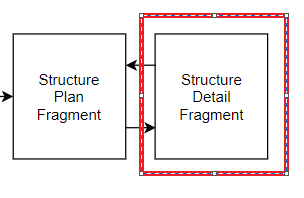
\includegraphics[width=1.0\textwidth]{images/06_AndroidApp/06_StructureDetailStellung}
\caption{Stellung des StructureDetaiFragment in der Android Applikation}
\label{fig:mediaNav}
\end{figure}
\\
In der Ressource Datei ''fragment\_structure\_detail.xml'' befindet sich eine ''TextView'' als einziges Element. Die ''onCreateView'' Methode der Klasse ''StructureDetailFragment'', wird nach Zuweisen der Layout Ressource, der Struktur beschreibende ''JSON-String'' aus dem ''Bundle'' gelesen. Dies geschieht über die Methode ''setArguments'' der Basisklasse Fragment und deren Feld ''mArguments'', und dem Anzeigefeld. Anschließend wird dem Fragment noch die Fähigkeit gegeben sich Scrollen zu lassen und die View wird zurückgegeben. 
\begin{lstlisting}[language=Java,caption={Übernahme und anzeigen der Daten im StructureDetailFragment}]
View v = inflater.inflate(
	R.layout.fragment_structure_detail, container, false);
Bundle bundle = this.getArguments();
TextView tvStructureDetailString = 													v.findViewById(R.id.tvStructureDetailString);
    
String detail = bundle.getString("actStructure");
    
tvStructureDetailString.setText(detail.toString());    tvStructureDetailString.setMovementMethod(
    new ScrollingMovementMethod());
\end{lstlisting}
\section{Request-Helper}
Um in weiterer Folge die Anfragen an den Java-EE-Server einfach und einheitlich durchzuführen, gibt es die Klasse ''RequestHelper'' . In dieser Klasse gibt es neben den beiden Parametern ''responseBody'' und ''responseCode'', welche zur Fehlerausgabe und zum Erhalt der Daten aus der Anfrage vorhanden sind, die Methode ''executeRequest''. Diese übernimmt die Hauptaufgabe der Klasse und führt die Anfragen an das Signage System durch. Werden Daten als Antwort der Anfrage erwartet so kann die Methode mit ''Callback'' Parameter aufgerufen werden. Ist dies nicht der Fall, so gibt es die Möglichkeit diese Methode ohne ''Callback'' aufzurufen. Dabei wird dieser Parameter mit dem Wert null überschrieben.
\\
Die Parameter dieser Methode lauten wie folgt:
\\
\begin{itemize}
	\item {\em RequestTypeEnum:} Der Parameter vom Typ Enum wird genutzt um herauszufinden welche Http Anfrage vorliegt. Mögliche Werte sind hierbei GET, POST, PUT und DELETE.
	
	\item {\em Params:} Hier liegt eine HashMap vor, die als Key-Value Paare alle benötigten Parameter für den RequestBody beinhaltet. Beispielsweise: ''LayoutID'':''78'', hierbei ist ''LayoutID'' der Key und ''78'' das Value.
		
	\item {\em Url:} Beinhaltet die URL unter der die Anfrage erreichbar ist. 
	
	\item {\em Callback:} Dieser Parameter wird benötigt, um auf eine Antwort des ausgeführten ''REST-Request'' zu warten. Wird ein ''Response'' erhalten und die Daten werden in dem angezeigten Fragment benötigt, können diese über eine ''Lamda-Expression'' in die gewünschten Anzeigeelemente eingefügt werden. 
\end{itemize}
Zu Beginn der Methode wird anhand des Parameters RequestTypeEnum unterschieden, um welche Http Anfrage es sich handelt. Wird GET oder DELETE geliefert, wird durch die HashMap iteriert und die einzelnen Key-Value Paare als QeryParameter in der URL einfügt.
Beispielsweise:''<URL>/layout?layoutID=78'' .
\begin{lstlisting}[language=Java,caption={GET oder DELETE Request}]
if (params != null && params.size() > 0) {
    Iterator it = params.entrySet().iterator();
    while (it.hasNext()) {
     	Map.Entry p = (Map.Entry) it.next();
	    urlBuilder.addQueryParameter(
	      	p.getKey().toString(), p.getValue().toString());
        }
    }
\end{lstlisting}
Handelt es sich um eine POST oder PUT Anfrage, so werden die Key-Value Paare im Body mitgegeben und im Format "application/x-www-form-urlencoded" codiert.
\begin{lstlisting}[language=Java,caption={POST oder PUT Request}]
String stringbody = "{";
if (params != null && params.size() > 0) {
  	Iterator it = params.entrySet().iterator();
    while (it.hasNext()) {
       	Map.Entry p = (Map.Entry) it.next();
        stringbody += "\"" 
        + p.getKey().toString() 
        + "\"" + ":" + "\"" 
        + p.getValue().toString() 
        + "\"" + ",";
        }
    }
stringbody = stringbody.substring(
  	0, stringbody.length() - 1);
stringbody += "}";
body = RequestBody.create(
MediaType.parse("application/json")
       			, stringbody);
\end{lstlisting}
Anschließend wird die URL mittels HttpUrl.Builder erstellt und ausgegeben. 
Des Weiteren wird per Switch-Case dem Request die richtige Art der Anfrage zugewiesen und danach die URL übergeben. 
\begin{lstlisting}[language=Java,caption={Zuweisung der Art der Anfrage}]
URL finalUrl = urlBuilder.build().url();
    Log.i(LOGTAG, "FinalUrl: " + finalUrl.toString());
    Request.Builder rb = new Request.Builder();
    switch (executeType) {
        case GET:
            rb = rb.get();
            break;
        case PUT:
            rb = rb.put(body);
            break;
        case POST:
            rb = rb.post(body);
            break;
        case DELETE:
            rb = rb.delete();
            break;
    }
\end{lstlisting}
Um die REST-Anfragen fertig zu stellen, wird das Interface Callback implementiert. Mit den beiden Methoden onFailure und onResponse wird dem Interface zugewiesen was passiert, wenn der Request fehlschlägt oder funktioniert. 
\\
\\
\textbf{onFailure:}
Sollte der Request fehlschlagen, wird im Log-Fenster der Responsecode und die Fehlermeldung/Exception ausgegeben. 
\\
\\
\textbf{onResponse:}
Wird der Request ohne Fehler durchgeführt so wird im Log-Fenster ebenfalls der Responsecode und der Responsebody ausgegeben. Letzter Schritt beim Erhalt des gewünschten ''Response'' ist es dem im Methoden Kopf übergebenen ''Callback'' Parameter auszuführen.
\\ 
\\
Der letzte Schritt ist dem OkHttpClient mitzuteilen, dass er einen neuen Call ausführen soll. Als Parameter wird der zusammengestellte Request mitgegeben. Über ''enqueue'' wird dem Client gesagt er soll auf einen Response warten. Parameter für diese Methode ist das erstellte Objekt vom Typ Callback.
\cite{OkHttp3}
\\
Um Daten aus den Requests zu erhalten beziehungsweise Fehlerausgaben anzeigen zu können gibt es Getter zu den Feldern ''responseBody'' und ''responseCode''. Verläuft der Request fehlerfrei so werden die geforderten Werte in die Variablen übertragen und können im weiteren Verlauf durch die Methoden ''getResponseCode'' beziehungsweise ''getResponseBody'' (Getter) ausgelesen werden. Im Fehlerfall wird lediglich der ''responseCode'' mit dem Fehlercode belegt und kann ausgelesen werden. 
\begin{lstlisting}[language=Java,caption={Getter und Setter für erhaltene Daten}]
public int getResponseCode() {
    return responseCode;
}

public void setResponseCode(int responseCode) {
    this.responseCode = responseCode;
}

public String getResponseBody() {
    return responseBody;
}

public void setResponseBody(String responseBody) {
    this.responseBody = responseBody;
}
\end{lstlisting}
\\
Antworten des Servers werden in Form von JSON-Strings erhalten. Das Aufbereiten dieser Daten wird den einzelnen Fragmenten, welche die Anfragen in Auftrag geben, überlassen, da die erhaltenen Informationen von Fragment zu Fragment verschiedene Inhalte aufweisen. 
\\
Um klarzustellen wie das Aufbereiten der Daten funktioniert wird anhand des Beispiels ''StructurePlanFragment'' gezeigt was passiert, sollte die Anfrage eine positive Antwort erhalten. Zu beachten ist, dass die Zuweisung der erhaltenen Daten in einer Lamda-Expression durchgeführt wird. Als erstes werden eine Liste von JSON-Objekten und ein JSONArray deklariert, um das Anzeigen und Durchlaufen der Informationen zu ermöglichen.
\begin{lstlisting}[language=Java,caption={Erstellen der benötigten Variablen}]
MainActivityBottomNavigation.getInstance().runOnUiThread(()->{
	LinkedList<JSONObject> structureparts = new LinkedList<>();
    JSONArray jsonArray = null;
\end{lstlisting}
Das Array wird hierbei zum Durchlaufen benötigt. Die LinkedList bildet die Quelle für die Anzeigedaten des Fragments. Da JSON-Strings im folgenden Abschnitt konvertiert werden ist ein try-catch block nötig, in dem mögliche Fehlerfälle behandeln und ausgegeben werden können. Die übermittelten Daten werden über den ''responseBody'' Getter ausgelesen und in das JSONArray übernommen. Über Iteration durch das JSONArray werden die einzelnen JSONObjekte ausgelesen und der LinkedList angehängt.
\begin{lstlisting}[language=Java, caption={Durchlauf des erhaltenen JSONStrings}
jsonArray = new JSONArray(rh.getResponseBody());
for (int i = 0; i < jsonArray.length(); i++) {
	JSONObject jsonObject = jsonArray.getJSONObject(i);
	structureparts.add(jsonObject);
}
\end{lstlisting}
 Nicht immer ist eine Iteration durch den Erhaltenen JSON-String nötig, beispielsweise bei der Anfragen in der der XIBO-Server-Status festgestellt wird. Im Anschluss werden die Anzeigeelemente mit den ausgelesenen Werten versehen, dabei ist zu beachten, dass dieser schritt über den UI-Thread ausgeführt wird da nach erzeugen der View die Anzeigeelemente verändert werden. 
\begin{lstlisting}[language=Java,caption={Zuweisung der Daten an das Anzeigeelement}]
StructurePlanAdapter structurePlanAdapter = 
	 	new StructurePlanAdapter(structureparts);
rvStructurePlan.setAdapter(structurePlanAdapter);
LinearLayoutManager linearLayoutManager = 
		new LinearLayoutManager(getContext());
linearLayoutManager.setOrientation(LinearLayoutManager.VERTICAL);
rvStructurePlan.setLayoutManager(linearLayoutManager);
\end{lstlisting}
\\